\begin{figure}[h]\centering
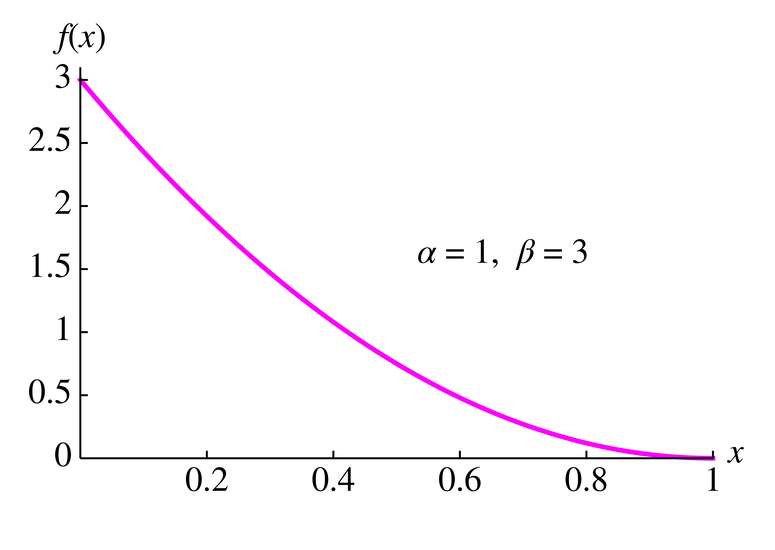
\includegraphics[width=.3\textwidth]{beta.png}
\caption{beta}
\end{figure}
\begin{figure}[h]\centering
    \includegraphics[width=.3\textwidth]{binominal.png}
    \caption{binominal}
\end{figure}
\begin{figure}[h]\centering
    \includegraphics[width=.3\textwidth]{epsilon_lambda.png}
    \caption{epsilon lambda}
\end{figure}
\begin{figure}[h]\centering
    \includegraphics[width=.3\textwidth]{gama.png}
    \caption{gama}
\end{figure}
\begin{figure}[h]\centering
    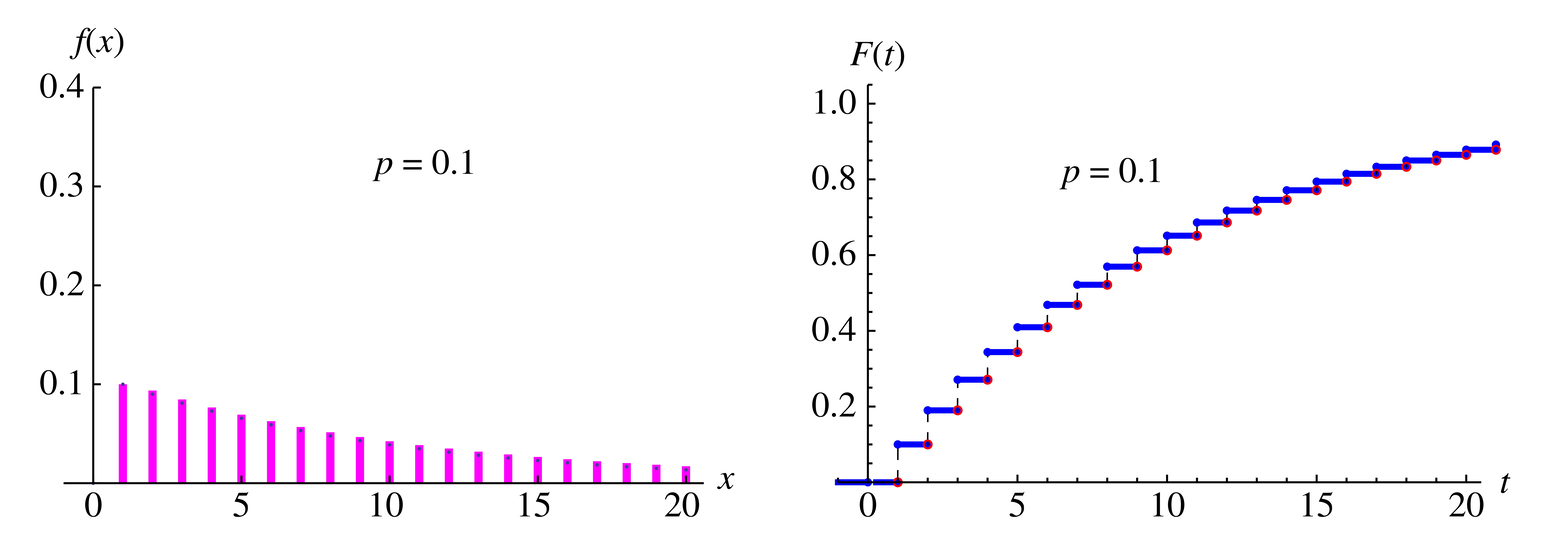
\includegraphics[width=.3\textwidth]{geom.png}
    \caption{geom}
\end{figure}
\begin{figure}[h]\centering
    \includegraphics[width=.3\textwidth]{hyperg.png}
    \caption{hyperg}
\end{figure}
\begin{figure}[h]\centering
    \includegraphics[width=.3\textwidth]{normal.png}
    \caption{normal}
\end{figure}
\begin{figure}[h]\centering
    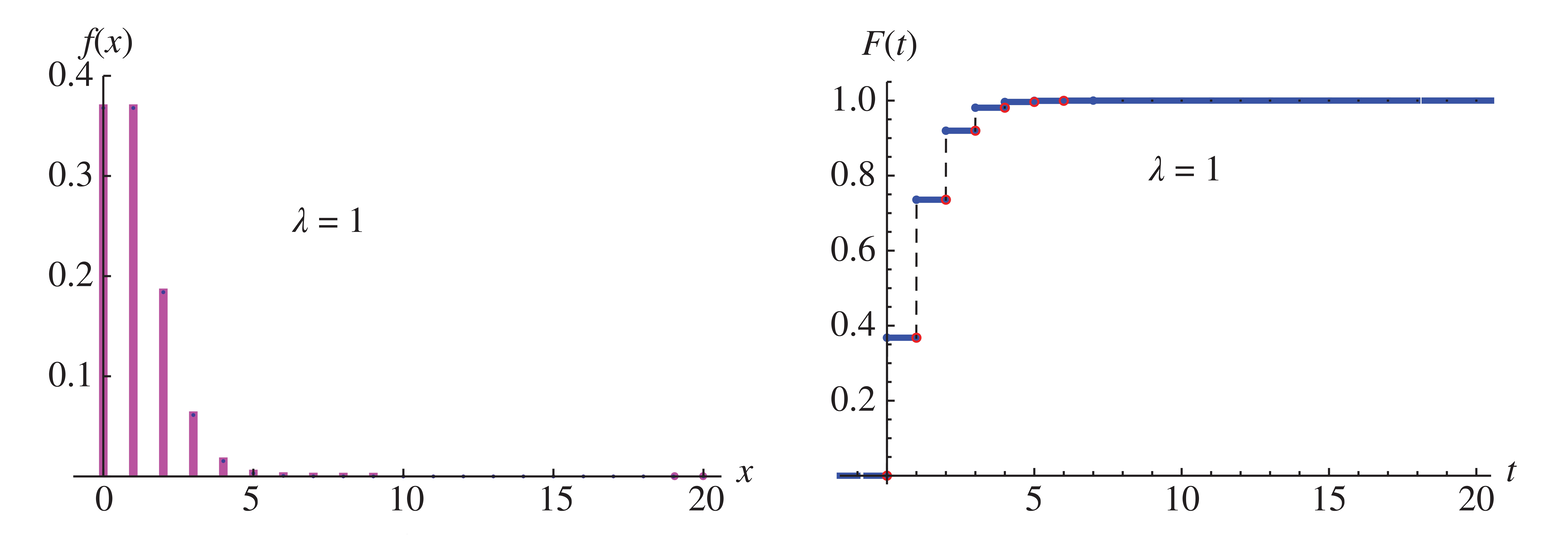
\includegraphics[width=.3\textwidth]{poisson.png}
    \caption{poisson}
\end{figure}

\begin{figure}[h]\centering
    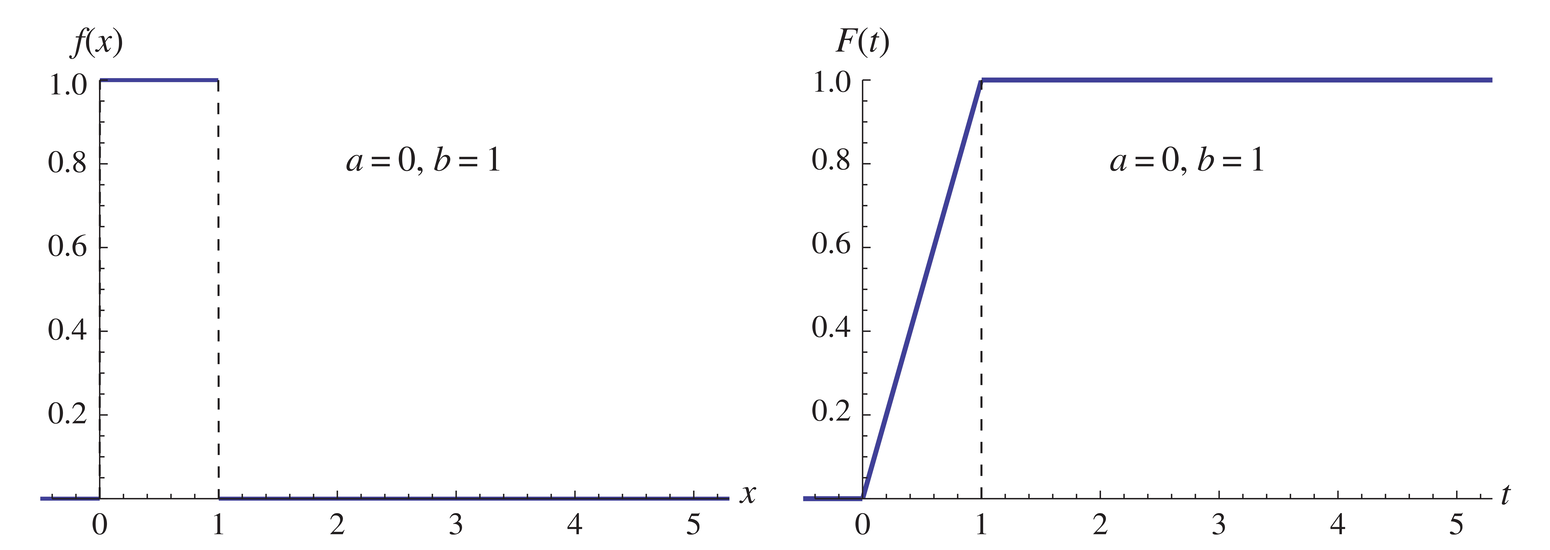
\includegraphics[width=.3\textwidth]{uniforme.png}
    \caption{uniforme}
\end{figure}
